\chapter{Bevezetés}
\label{ch:intro}

A fordítóprogramok feladata a magas szintű programkód átalakítása a számítógép számára értelmezhető formára. Céljuk, hogy a programozó sokkal magasabb absztrakciós szinten fejezhesse ki szándékát, ezáltal megkönnyítve a szoftverfejlesztés folyamatát. A kódvisszafejtő programok működése ezzel ellentétes, az alacsony szintű, gépközeli kódot alakítják át magas szintű kóddá. Segítségével beleláthatunk a program forráskódjába akkor is, ha csak egy futtatható állomány áll rendelkezésre, ezáltal könnyebben megvédhetjük gépünket a kártékony szoftverektől.

A fenti feladat megoldására már léteznek különböző kódvisszafejtő programok \cite{ghidra, binaryninja}, ugyanakkor ezek legnagyobb hátránya, hogy a fordítóprogramokhoz hasonlóan bonyolult szabályok alapján működnek. Ez azért probléma, mert ezen szabályokat minden programozási nyelv esetén külön meg kell fogalmazni, ami egy bonyolult és időigényes feladat.

Dolgozatomban egy olyan programot mutatok be, ami a fenti problémát a természetes nyelvfeldolgozásban használt gépi tanulási eszközökkel oldja meg. A neurális gépi fordítás az utóbbi években hatalmas fejlődésen ment keresztül[bert], így könnyen adódik, hogy ezen eredményeket fel lehetne használni a kódvisszafejtéshez, annyi különbséggel, hogy nem angolról németre, hanem például assembly-ről C-re fordítunk.\footnote{Majd látni fogjuk, hogy a programozási nyelvek sajátos szerkezete miatt sajnos nem alkalmazhatók egy az egyben a természetes nyelvek fordítása során elért eredmények.} Ezen módszer előnye, hogy nem szükséges hozzá programozók hosszú ideig munkája a különböző szabályrendszerek megalkotásához, valamint egy másik nyelvre való áttérés sem okoz különösebb nehézséget. Továbbá a különböző programkód generáló szoftvereknek\cite{??} hála, lényegében korlátlan mennyiségű adat áll rendelkezésre.

\section{A kódvisszafejtés lépései}
A kódvisszafejtés három fő lépésben történik, ezek közül az első kettőben
használtam neurális hálókat. Nulladik lépésként az Assembly kód kinyerése
történik a futtatható állományból, erre az \texttt{objdump} eszközt használtam.

\subsection{Assembly szegmentálás}
A visszafejtés első lépésében történik az Assembly kód szegmentálása, ahol
a cél, hogy úgy daraboljuk fel a kódot egymás utáni blokkokra, hogy egy-egy ilyen blokk egy
sor C kódnak feleljen meg. Ehhez egy \texttt{LSTM}\cite{lstm} cellákból álló
rekurrens neurális hálót használok. (TODO: Ábra) A modell bemenete az Assembly sorok,
a kimenete pedig minden sorra $1$, ha ott kezdődik egy blokk, $0$ egyébként. Ez
egy bináris klasszifikációs probléma, melyet a modell könnyedén megtanult.

\subsection{Maszkolt C kód előállítása}
A második lépésben minden Assembly blokkot egy sor C kódnak próbálunk
megfeleltetni. Fontos, hogy ebben a lépésben nem várjuk el a változók és
a számliterálok pontos visszaállítását. Ezért az eredeti C kódban minden
változó előfordulást \texttt{VAR}-ra, minden számliterál előfordulást
\texttt{NUM}-ra cserélünk. A konkrét értékek visszahelyettesítése majd
a harmadik lépésben fog megtörténni.

Ezen probléma megoldására egy enkóder-dekóder modellt használtam. Az enkóder
első lépésben a bemeneti Assembly blokk sorait kódolja egy vektorba, majd
a dekóder ezen vektorból állítja elő a kimeneti tokenek listáját. A lehetséges
kimeneti tokeneket a ?? táblázat tartalmazza.

\subsection{Változók és számliterálok rekonstruálása}
A harmadik lépésben minden előállított maszkolt C sorra megpróbáljuk
visszaállítani, hogy konkrétan milyen változók\footnote{A konkrét változónevek
elvesznek a fordítás során, így ezeket nem lehet visszafejteni, ezért itt
annyit követelünk meg, hogy két változó ugyanaz-e vagy sem.} és milyen
számliterálok szerepeltek ott. Ezeket soronként, a hozzá tartozó Assembly blokk
segítségével próbáljuk rekonstruálni, az alábbi lépésekben:
\begin{enumerate}
    \item Változók és számliterálok kinyerése a megfelelő Assembly blokkból
    \item Ezek permutálása és behelyettesítése a \texttt{VAR} és \texttt{NUM}
    tokenek helyére
    \item Az eddig rekonstruált és a mostani behelyettesítésből kapott kódrészlet lefordítása
    \item Ha a lefordított Assembly megegyezik\footnote{Teljes egyezést nem
    várhatunk el, hiszen lehet, hogy pl. más regiszterekre hivatkozunk, ezért
    csak "szerkezeti" egyezést követelünk meg.} az eredeti Assembly-vel, akkor
    lépünk a következő blokkra, különben visszalépünk a $2.$ pontra.
\end{enumerate}
Így sorról sorra behelyettesítjük a változókat és számliterálokat, így végül
visszanyerjük az eredeti\footnote{A változónevek $x0,x1,\dots$ lesznek}
C kódot.
\subsubsection{Probléma a szorzással, osztással és modulozással}
Az \texttt{x0 = x1 + 5 ;} kifejezésnek megfelelő Assembly blokkban 
megjelenik az $5$-ös számliterál, ugyanakkor ez nem minden műveletnél van így.
Hatékonysági okokból a számmal való osztás során a fordító nem osztást fog
generálni, hanem szorzást és bitshifteléseket. Ezért például a $17$-tel való
osztás során a vonatkozó Assembly blokkban megjelenő számliterálok a $[...]$.
Láthatjuk, hogy $17$ ezek között nincs ott, ezért hiába próbáljuk végig
a behelyettesískor az összes számliterált, soha nem fogjuk a megfelelő Assembly
blokkot visszakapni.

Ezen probléma megoldására előre regeneráltam, hogy egy adott számmal való
osztás során milyen "varázsszámok" jelennek meg az Assembly-ben. Ezután a fenti
algoritmus még kiegészítésre kerül annyiban, hogy nem csak az Assembly-ben
megjelenő számliterálokat próbáljuk behelyettesíteni a \texttt{NUM} tokenek
helyére, hanem ha pl. a $[...]$ számok mind szerepelnek, akkor ehhez a listához
a $17$-et is hozzávesszük.

A szorzás és modulozás során hasonló probléma lép fel, például a $[...]$
számokkal való szorzás esetén egyáltalán nem jelenik meg számliterál az
Assembly-ben. Így ezeket mindig hozzá kell venni a lehetséges számliterálok
listájához, ha van a kifejezésben \texttt{*} token.

A hátránya ennek a módszernek, hogy ha egy kifejezésben több \texttt{/},
\texttt{\%} vagy \texttt{*} token van, akkor a lehetséges számliterálok száma
nagyon megnő, ezáltal a program futási ideje is sokkal nagyobb lesz, mivel
minden lehetséges behelyettesítés kipróbálása során le kell fordítani
a kapott programot.

\begin{figure}[H]
	\centering
	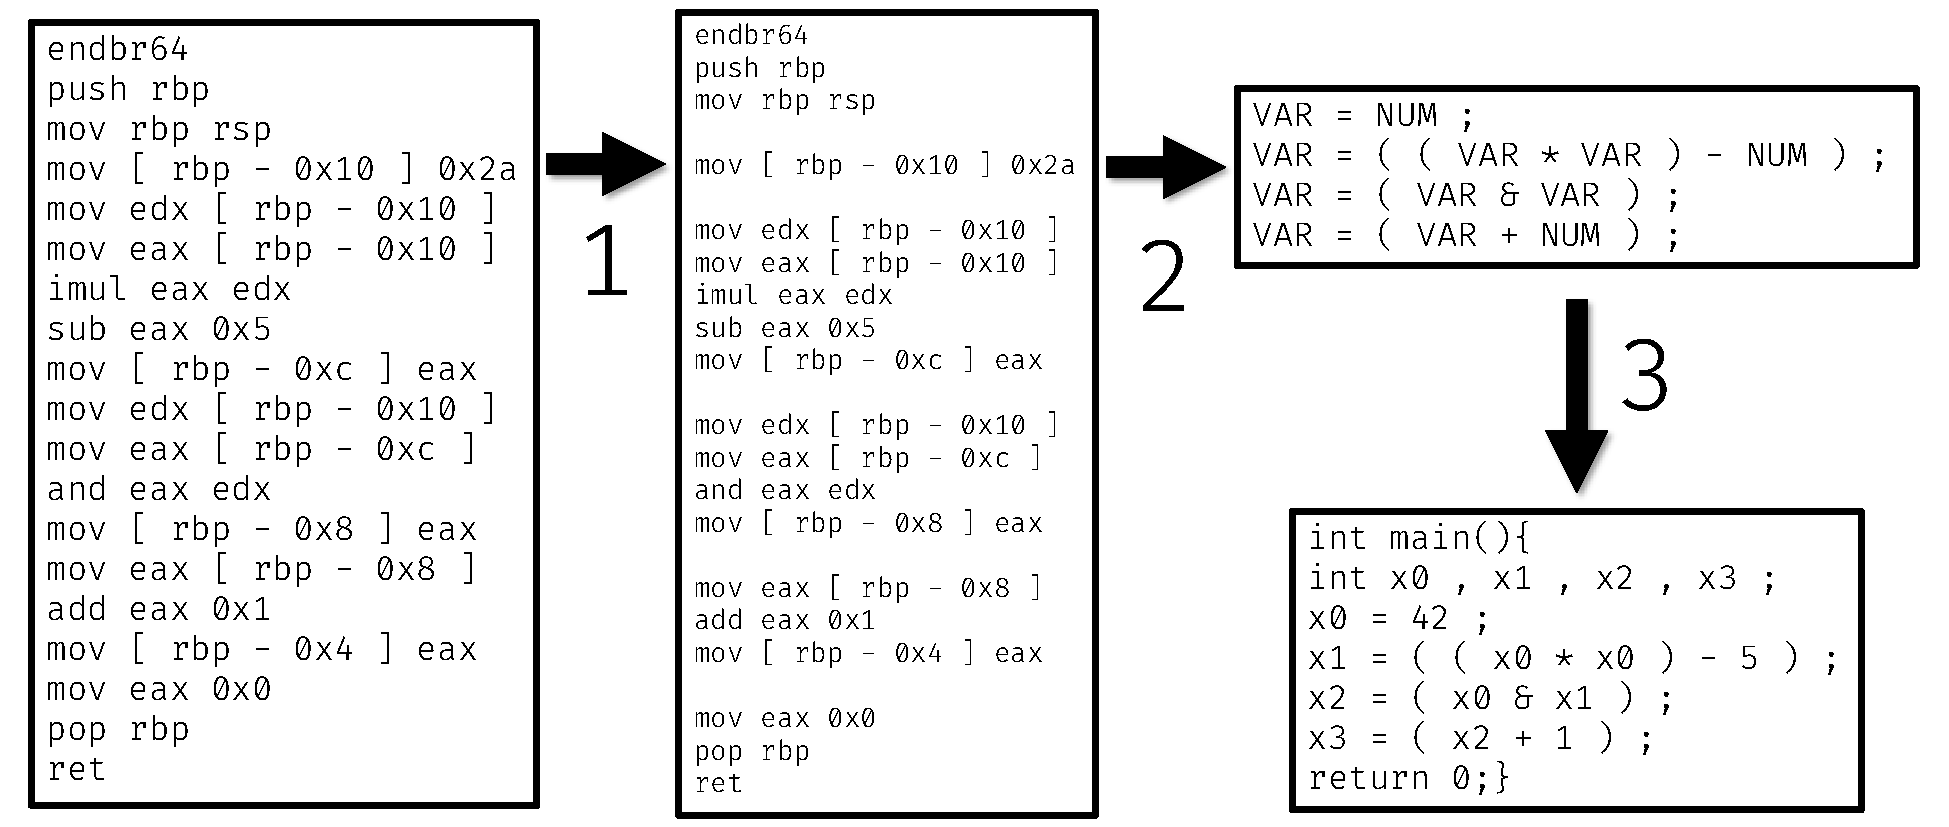
\includegraphics[width=1\textwidth]{images/steps.pdf}
	\caption{A kódvisszafejtés lépései}
	\label{fig:steps}
\end{figure}

\subsection{Assembly beágyazás}
Az első két lépésben használt modellek valójában nem a nyers Assembly sorokat
kapják meg bemenetként, hanem az azokból előállított kontextusvektorokat. Ez
a trükk már régóta ismert a neurális gépi fordítási problémák megoldása során,
a legismertebb ilyen megoldás a \texttt{Word2Vec}\cite{word2vec}. Ahhoz hasonlóan az
Assembly beágyazásnál is cél, hogy a hasonló soroknak közeli vektorokat
feleltessünk meg, ezzel megkönnyítve a későbbik során a modell tanulási
folyamatát. Én erre a problémára a \texttt{Palmtree}\cite{palmtree} eszközt használom. Ez
minden sor Assembly-t egy \texttt{N} dimenziós vektorba képez le. Működési elve
a \texttt{BERT}\cite{bert}-höz hasonló.
